\subsection{Kirchhoffsche Regeln}
    \subsubsection{Knotenregel}
        \vspace{-1mm}
        \begin{minipage}{0.49\linewidth}
            \begin{footnotesize}
                \begin{center}
                    \vspace{2mm}
                    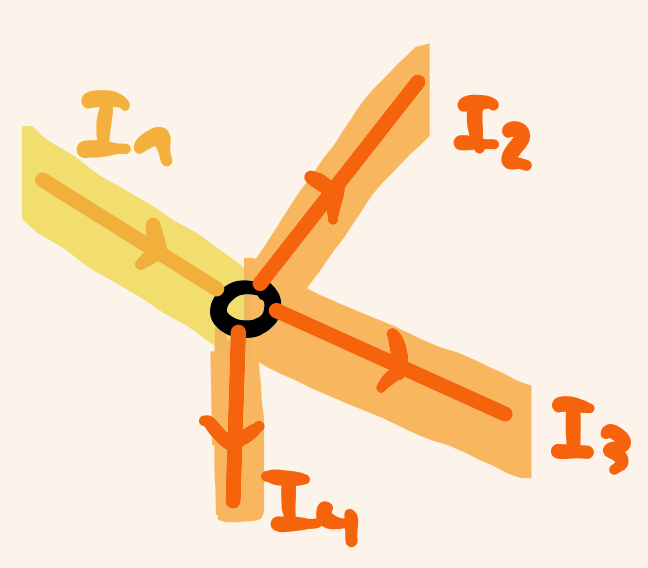
\includegraphics[width = 20mm]{src/images/knotenregel.png}
                \end{center}
            \end{footnotesize}
        \end{minipage}
        \begin{minipage}{0.5\linewidth}
            \begin{scriptsize}
                \begin{center}
                    \begin{align*}
                        \text{Widerstände:} \; &\sum\limits_k I_k = 0\\
                        \text{Kondensatoren:} \; &\sum\limits_k Q_k = 0
                    \end{align*}
                    \colorbox{Goldenrod}{$\sum I_\text{zufliessend}$} $=$ \colorbox{Apricot}{$\sum I_\text{abfliessend}$} 
                \end{center}
            \end{scriptsize}
        \end{minipage}
        \vspace{1mm}

    \subsubsection{Maschenregel}
        \vspace{-1mm}
        \begin{minipage}{0.49\linewidth}
            \begin{footnotesize}
                \begin{center}
                    \vspace{2mm}
                    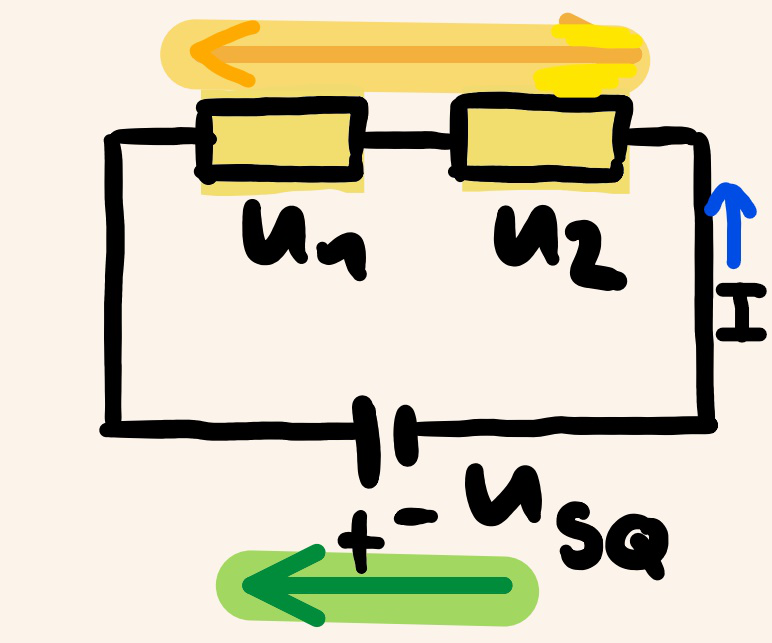
\includegraphics[width = 20mm]{src/images/maschenregel.png}
                \end{center}
            \end{footnotesize}
        \end{minipage}
        \begin{minipage}{0.5\linewidth}
            \begin{scriptsize}
                \begin{center}
                    \begin{align*}
                        \text{Widerstände:} \; &\sum\limits_{i} U_{i} = \sum\limits_k R_k I_k \\
                        \text{Kondensatoren:} \; &\sum\limits_{i} U_{i} = \sum\limits_k \frac{Q_k}{C_k} 
                    \end{align*}
                    $i =$ \# Spannungsquellen\\
                    $k =$ \# Spannungsabfälle
                \end{center}
                \vspace{1mm}
                \hfill \colorbox{YellowGreen}{$\sum U_\text{Quelle}$} $=$ \colorbox{Yellow}{$\sum U_\text{Abfälle}$} 
            \end{scriptsize}
        \end{minipage}
        \begin{scriptsize}
            (1) Zeichne \colorbox{YellowGreen}{$\vec{U}_{sq}$}an der Spannungsquelle ein (minus nach plus)
            \\(2) Wähle Stromrichtung \colorbox{Cyan}{$\vec{I}$} (gegen $U_{sq}$)
            \\(3) Trage \colorbox{Yellow}{$\vec{U}_R$} an Widerständen (ein gleich wie Stromrichtung)
        \end{scriptsize}